\section{Design of the Solution}

\label{sec:design}


\subsection{Requirements and Assumptions }

% A table 

The design of the platform was made having the following assumptions:

P1 - Crowdsourcing: community wisdom works for big numbers better than individual wisdom

P2 - Incentives: If there are enough incentives, community contributes

P3 - A new developer is always an unkown developer

P4 - The Apps from a Trusted Developer are Trusted Apps

P5 - In a dispute, if 50\% + 1 of the community is honest, the right side wins

P6 - Transactions registered in the blockchain ledger (IAB, Ads) reflects well the trustworthness of a developer.

P7 - If the app downloads made by the users come from more than 5\% of unknown developers, users will start to trust in unknown developers.

P8 - A community dispute may take 30 days. While the dispute is handled, the app stores have the option of hiding the app to avoid zero-day attacks.


\subsection{Client side support}

Besides the blockchain technology, the environment where the user is running the app store, should also support app coins protocol.

% TODO : include quote

As Android represents 86\% of the smartphones market, we focus an implementation analysis in that platform. However, many of the constraints and solutions are applicable to other smaprthone operating systems.

This sub-section\footnote{This section was contributed by Marcelo Benites, Aptoide Android team member} aims to describe client-side, at the smartphone untrusted environment, the method to register that an user is paying attention to an Application (installed from an App Store) for a certain amount of time. Once those requirements are met, a Proof-of-Attention is requested and stored at the blockchain.

\begin{itemize}
\item {\bf App store}: proof-of-attention compliant App Store Android application.
\item {\bf Application}: android application installed from App Store.
\item {\bf User}: user registered in App Store.
\end{itemize}

When designing a solution two main factors should be taken into account: reliability and availability. Reliability consists in avoiding fraud. Once a Proof-of-Attention is generated it has to be a high level of confidence that a User paid attention to an Application installed from an App Store. Availability consists in making sure whenever a User pays attentions to an Application installed from an App Store the App Store will be aware of that and will request the Proof-of-Attention once the requirements are met.

App Store process has to be running when User is paying attention to an Application in order to request  the Proof-of-Attention. Latest releases of Android operating system (Android OS) - from Lollipop (API level 21) onwards - have been limiting the ability of application processes to run while application is in background. In our scenario the App Store process could eventually be killed by the Android OS while not in foreground. In order to overcome that issue we will take advantage of the Binder framework to bind Application and App Store processes while Application is in foreground which will ensure App Store process is not killed by the Android OS.

\begin{figure}[!ht]
\centering
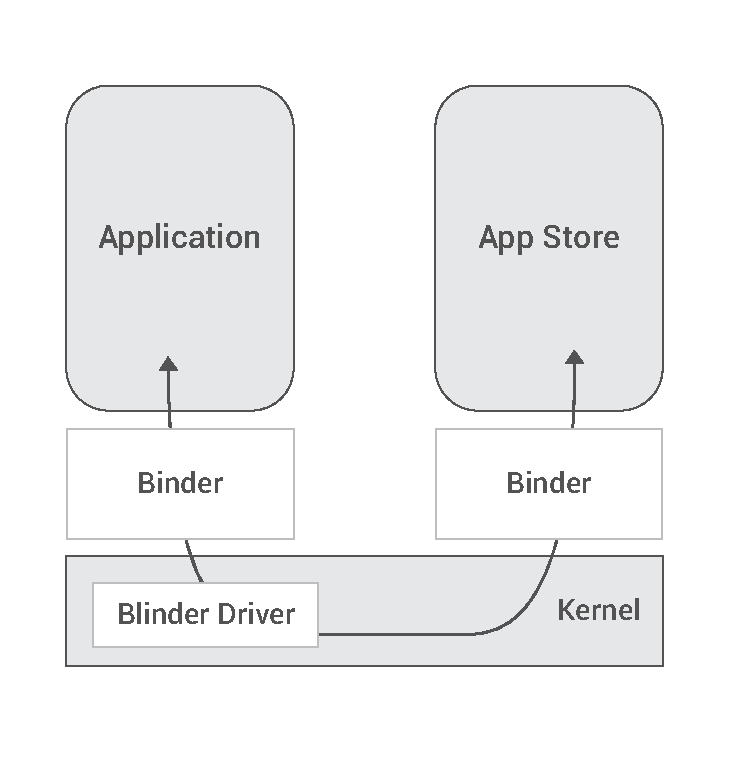
\includegraphics[width=0.5\textwidth]{diagrams/binder_diagram.eps}
\caption{Operating system binder.}
\label{fig:binder}
\end{figure}

Binder framework is a core component in Android architecture and its main goal is to simplify Inter-Process Communication (IPC). Binder is implicitly used whenever an application communicates with OS services or with other applications through Android Java API Framework. The Binder framework will also provide information regarding the Application process which will positively contribute to App Store Proof-of-Attention reliability.

Once Application and App Store processes are bound, App Store will periodically verify whether the Application is in foreground and the User is actively interacting with the device. In order to certify User is paying attention to the Application the following conditions should be met:

\begin{itemize}
\item Application process must be bound to App Store process.
\item The Application must be in foreground.
\item Device screen must be on.
\item Device must not be locked. 
\item The signature of the Application must be verified on App Store servers.
\end{itemize}

To assure Application process is bound to App Store, Binder and PackageManager APIs can be used. To verify whether Application process is in foreground ActivityManager, UserStatsManager and PackageManager APIs can be used. To check whether device screen is on PowerManager and Display APIs can be used. Regarding the state of the lock screen KeyguardManager API can be used. 

Every application has to be signed by the developer to be installed in an Android device. App Stores have access to the Applications signatures and can validated whether they match with the signature on their servers. If signature does not match Application may be tempered. To obtain the Application signature Binder and PackageManager APIs can be used.

\subsubsection{Limitations client-side}

The proposed solution has some limitations regarding reliability - imposed by Android inherently insecure environment - and Android API availability - due to Android version fragmentation and App Store permission level. The use of several different Android APIs can help hardening the solution against an attacker but can not assure full protection against fraud on the client side. In order to mitigate fraud a system has to have different security layers from client side to server side. 

In Android some APIs are considered sensitive and require system-level permissions to access them. Usually system-level can only be granted to system applications (pre-installed on the device by manufacturers). Also some APIs are only available in certain versions of Android. The following table summarizes the APIs needed to generate the Proof-of-Attention and their availability:


\begin{figure}[!ht]
\centering
\includegraphics[width=\textwidth]{diagrams/table_android_limitations.eps}
\caption{Table of Android versions and API support}
\label{fig:android_versions}
\end{figure}

The ``UsageStatsManager'' requires a System-Level permission but PACKAGE\_USAGE\_STATS can also be obtained if user explicitly enables it in Settings by a normal application.

We can only have an implementation that fulfills all the requirements to certify User is paying attention to the Application with a minimum Android version of Jelly Bean (API 16) and above. The Android version limitation is not relevant since according to Google statistics only 1.2\% of the Android devices are not running version Jelly Bean (API 16) or above. 

Also UsageStatsManager is necessary from Lollipop (API 21) onwards what will require App Store application to be a system application or to ask the user to explicitly go to Settings and give the permission. Since in the App Economy the User will be rewarded by the attention given to Applications it will be easy to convince him to manually provide the permission in case App Store is not a system application.


\subsection{Protocol Overview and sketch}

% a diagram that integrates all the players
% the circular but more geek 

%(Include a diagram with the players - component diagram 

% Could be a sequence diagram as in Filecoin diagram 

% (In-App Billing, Advertising, Reputation builder) 

%


